\chapter{Simulation numérique}

    \section{Introduction}
    La simulation numérique repose sur des outils mathématiques et algorithmiques pour transformer des équations différentielles en solutions approchées, fournissant ainsi un aperçu précieux sur des systèmes temporels. Ce chapitre introduit deux bibliothèques Python incontournables pour le calcul scientifique et la résolution numérique: \codeword{Numpy} pour la manipulation efficace des données et \codeword{SciPy} pour l'intégration numérique et la résolution de systèmes dynamiques.

    \section{Introduction à \texttt{Numpy}}
        \codeword{Numpy}, abréviation de \textit{Numerical Python}, est une bibliothèque qui s'est imposée dans le domaine du calcul scientifique (\cite{Numpy2020}). Elle propose des structures de données optimisées et un riche ensemble de fonctions mathématiques, rendant les manipulations et les calculs de tableaux multidimensionnels performants, en s'appuyant sur la notion de parallélisation. 

        \subsection{Pourquoi utiliser \texttt{Numpy} ?}
            L'un des principaux attraits de \codeword{Numpy} réside dans son efficacité. Les tableaux \codeword{Numpy} (appelés \codeword{ndarrays}) surpassent largement les listes natives de Python en termes de performance, en particulier pour la manipulation de grands ensembles de données. Cette performance est le fruit d'une implémentation sous-jacente en \codeword{C}, permettant à \codeword{Numpy} de bénéficier de la puissance du calcul vectorisé. Le calcul vectorisé, au lieu de traiter les éléments un par un, applique des opérations sur l'ensemble des éléments d'un tableau en une seule commande. En évitant les boucles explicites, \codeword{Numpy} offre un gain de vitesse significatif et rend le code plus lisible et compact.

        \subsection{Comment utiliser \texttt{Numpy} ?}
            Pour exploiter pleinement le potentiel de \codeword{Numpy}, il est essentiel de comprendre ses principales fonctionnalités. Nous introduisons des exemples pratiques, couvrant la création, la manipulation et l’application de fonctions mathématiques sur les tableaux.

            \subsubsection{Création et manipulation de tableaux}
                La création de tableaux est au cœur de l'utilisation de \codeword{Numpy}. Voici un exemple basique de création et manipulation d'un tableau \codeword{Numpy}:
                \inputminted{python}{codes/np_array.py}

            \subsubsection{Fonctions mathématiques vectorisées}
                \codeword{Numpy} permet l’application simultanée de fonctions mathématiques standards à chaque élément d’un tableau. Ce comportement vectorisé confère aux fonctions mathématiques de \codeword{Numpy} une grande efficacité, comme illustré ci-dessous:
                \inputminted{python}{codes/np_math.py}
            
            \subsubsection{Génération de séquences et nombres aléatoires}
                \codeword{Numpy} propose des fonctions pré-établies pour la génération de séquences arithmétiques et de nombres aléatoires, qui sont des outils précieux pour l'initialisation de simulations:
                \inputminted{python}{codes/np_init.py}
                \inputminted{python}{codes/np_random.py}
            
            \subsubsection{Calcul matriciel et multiplication matricielle}
                En plus de la manipulation de tableaux, \codeword{Numpy} dispose d’outils pour les calculs matriciels:
                \inputminted{python}{codes/np_matrix.py}
                Si la multiplication doit être matricielle:
                \inputminted{python}{codes/np_matmul.py}
    \section{Solveur numérique}
        Pour résoudre les systèmes dynamiques, nous utiliserons la fonction \codeword{solve_ivp} du module \codeword{integrate}, dans la librairie \codeword{SciPy} (\cite{Scipy2020}). Cette fonction intègre numériquement des équations différentielles. \robin{Tu peux faire le lien avec les algorithmes de type Runge-Kutta (fonctionnement par défaut de \texttt{solve\_ivp}) qui sont vus en F205.} Elle prend en paramètres:
        \begin{itemize}
            \item \textbf{La fonction à intégrer} : une fonction Python définissant l’équation différentielle.
            \item \textbf{L'intervalle de simulation} : la durée de la simulation.
            \item \textbf{Les points de discrétisation} : un \codeword{numpy.ndarray} définissant les points temporels pour lesquels la solution sera évaluée.
        \end{itemize}

    \section{Simulation de systèmes d'ordre 1}
        Dans cette section, nous explorerons des exemples classiques de systèmes d'ordre 1, résolus numériquement à l'aide de \codeword{SciPy}. Ces exemples sont plus simples que ceux abordés dans le chapitre \ref{chap:portrait_phases}, mais ils permettent de se familiariser avec la syntaxe qu'imposent \codeword{Numpy} et \codeword{SciPy}.
    
        \subsection{Intégrateur simple}
            Nous commençons par un modèle d'intégrateur simple, décrit par le système suivant \robin{à nouveau $y(t)=x(t)$, je ne comprends pas la notation.} \robin{Utilisation de 'prime' pour une dérivée (temporelle) alors que 'point' était utilisé jusqu'ici.}:
            \begin{equation*}
                \begin{cases}
                    x'(t)=c\,u(t)\\
                    y(t)=x(t)
                \end{cases}
            \end{equation*}
            avec les conditions initiales suivantes :
            \begin{itemize}
                \item Condition initiale: $x(0)=1$,
                \item Valeur du paramètre: $c=1$,
                \item Intervalle temporel: $[0,10]$,
                \item Entrée: $u(t)=\sin(t)$.
            \end{itemize}

            \subsubsection{Solution numérique}
                Le code suivant résout numériquement le système et affiche le résultat via la bibliothèque \codeword{Matplotlib} (\cite{Matplotlib2007}). Le graphique est présenté en Figure \ref{fig:integrateur_simple}. \robin{P-ê mentionner que la solution au système est $x(t) = 2-\cos t$ pour confirmer visuellement la solution~?}
                \inputminted{python}{codes/integrateur_simple.py}
                \begin{figure}[ht!]
                    \centering
                    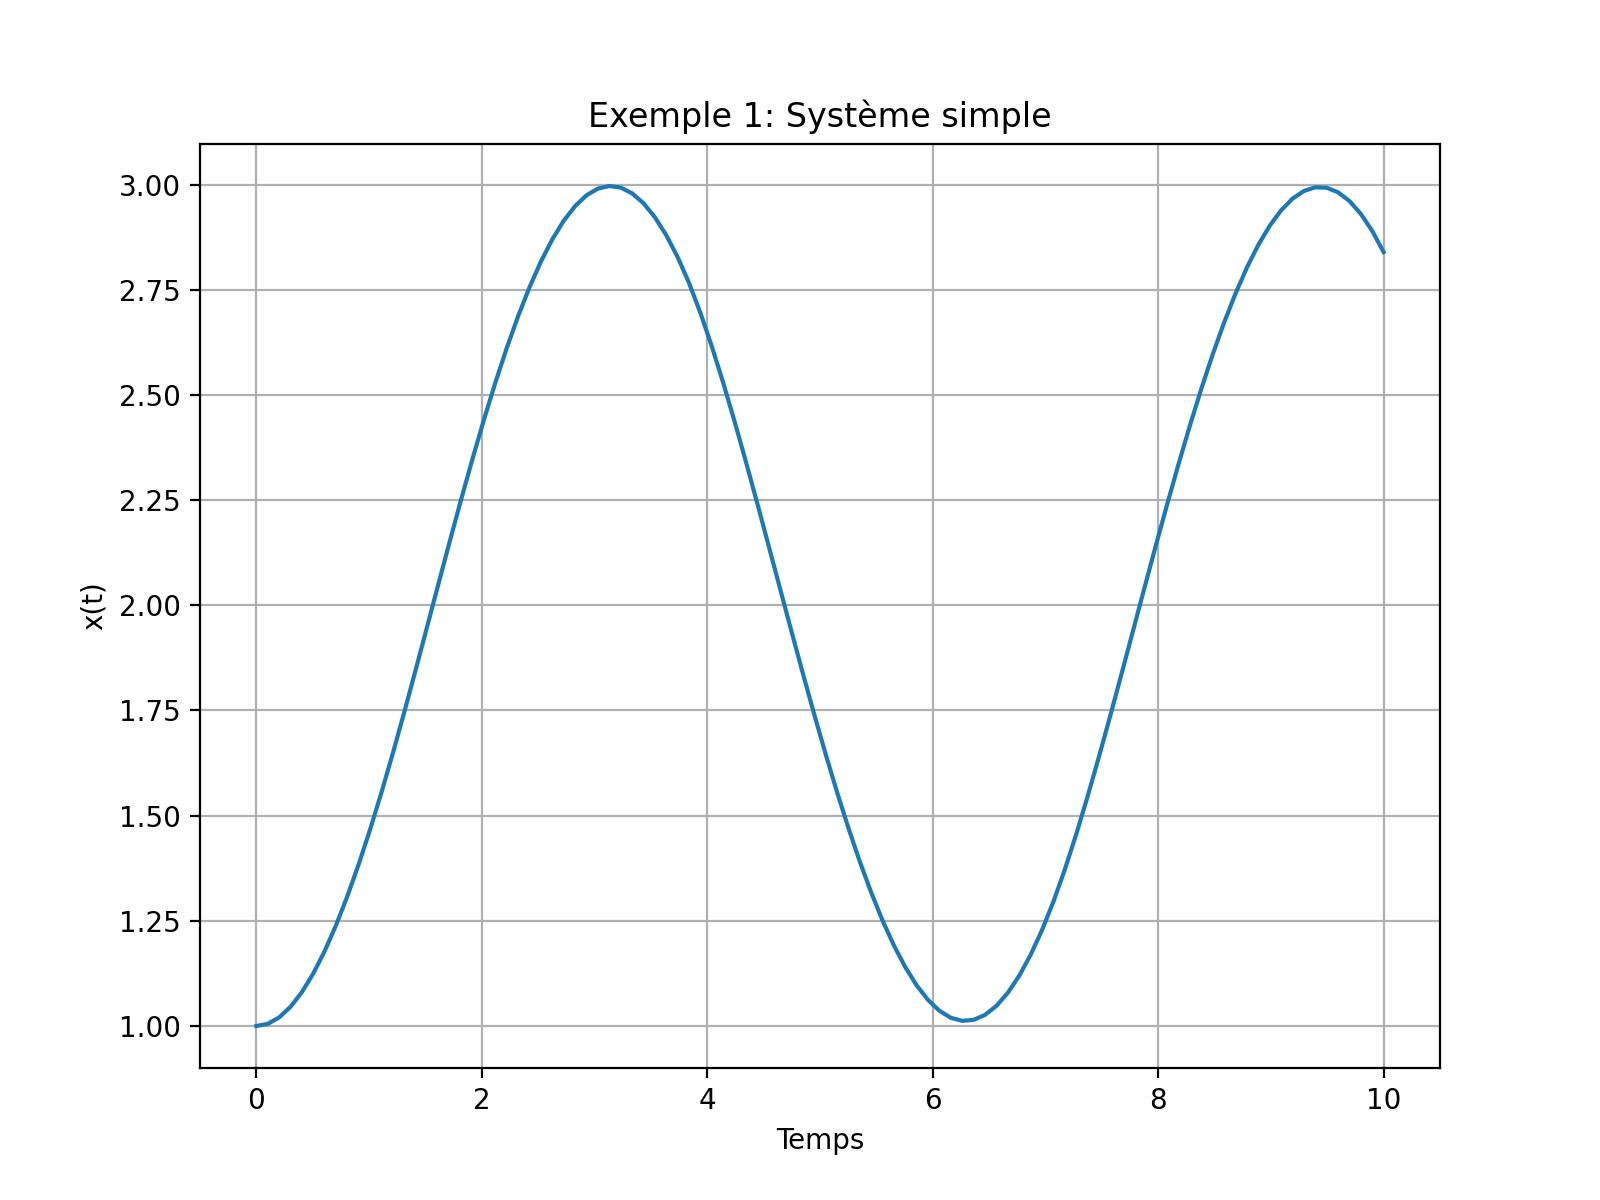
\includegraphics[width=\textwidth]{images/integrateur_simple.jpg}
                    \caption{Solution numérique de l'intégrateur simple}
                    \label{fig:integrateur_simple}
                \end{figure}

        \subsection{Croissance et décroissance exponentielle}
            Ce modèle a déjà été présenté dans le chapitre \ref{chap:equadiff}, dans lequel nous avons déterminé la solution analytique. Nous montrons que cette solution peut être aussi obtenue numériquement. Le système est décrit par
            \begin{equation*}
            \begin{cases}
            x'(t)=c\,x(t)\\
            y(t)=x(t)
            \end{cases}
            \end{equation*}
            avec les conditions suivantes :
            \begin{itemize}
                \item Condition initiale: $x(0)=1$,
                \item Valeur du paramètre: $c=0.1$,
                \item Intervalle temporel: $[0,10]$.
            \end{itemize}
        
            \subsubsection{Solution numérique}
                Ce code résout le système exponentiel et affiche le graphique de la solution en Figure \ref{fig:croissance_exponentielle}. \robin{Again, faire le lien avec la solution $x(t) = \exp(t/10)$~?}
                \inputminted{python}{codes/croissance_exponentielle.py}
                \begin{figure}[ht!]
                    \centering
                    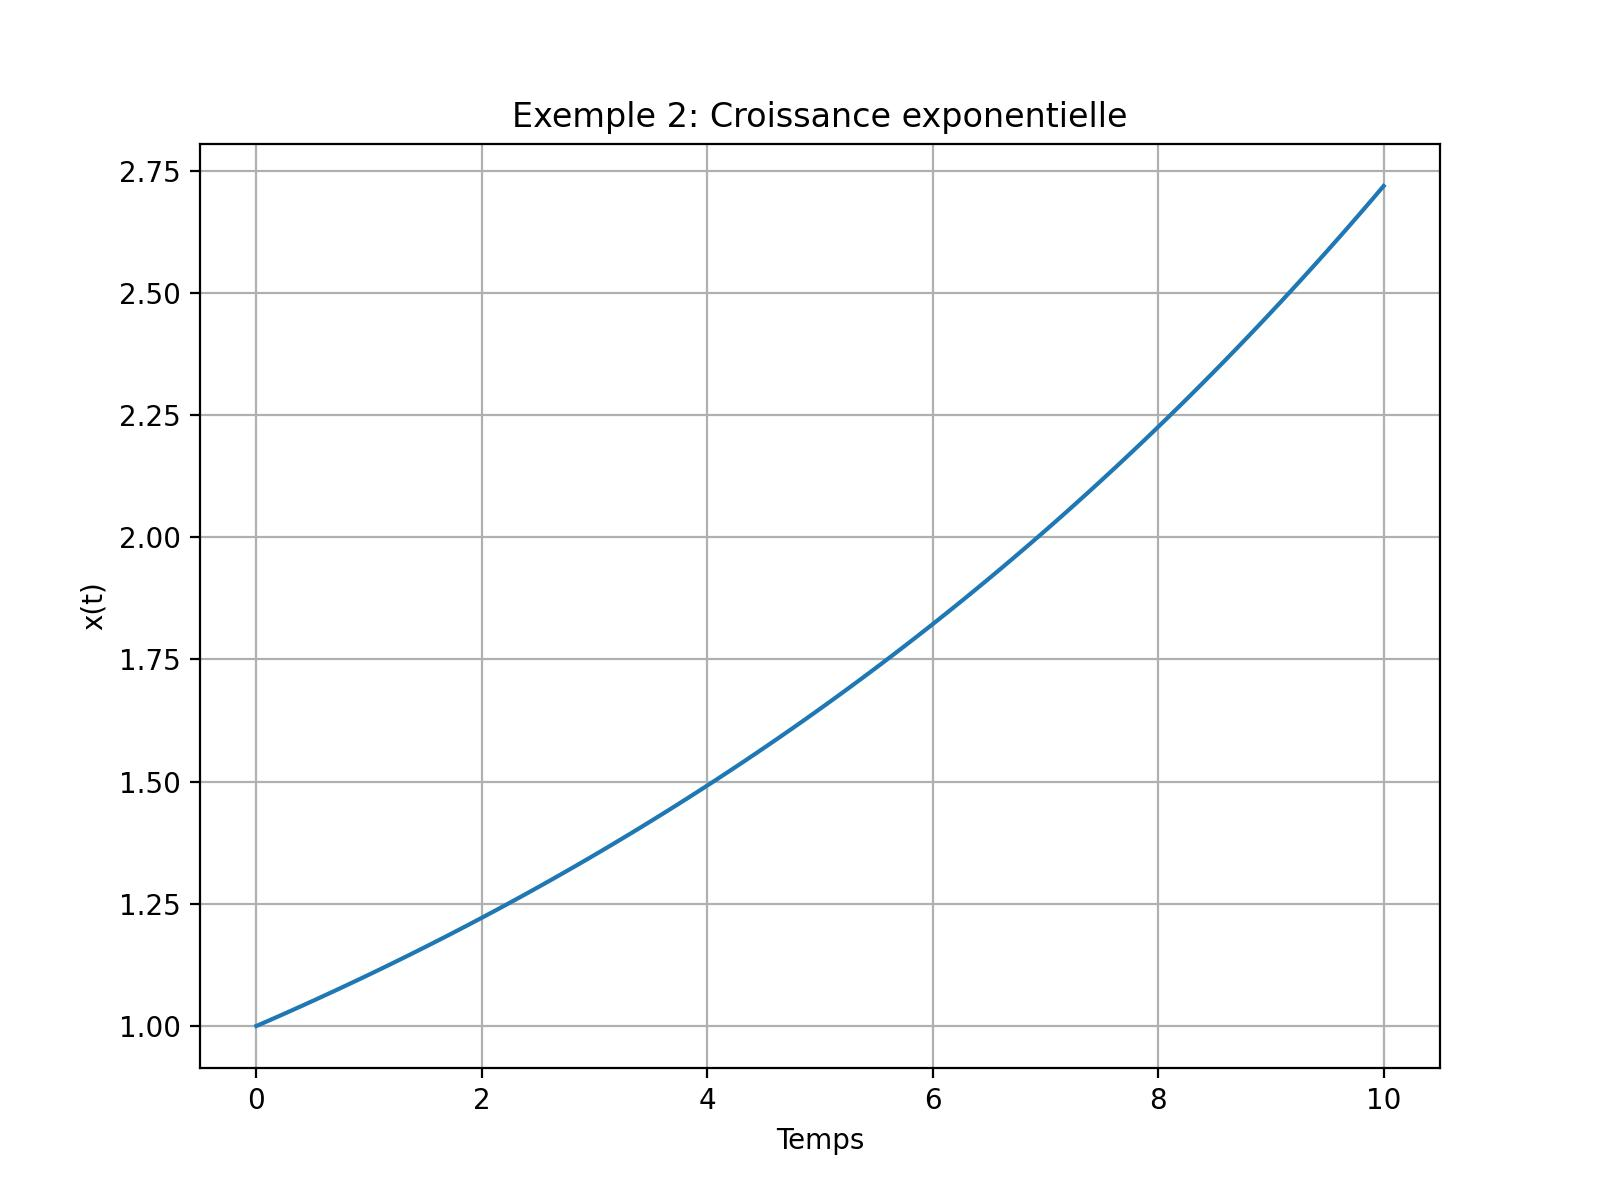
\includegraphics[width=\textwidth]{images/croissance_exponentielle.jpg}
                    \caption{Solution numérique de la croissance exponentielle}
                    \label{fig:croissance_exponentielle}
                \end{figure}

        \subsection{Système avec retard d'ordre 1}
            Pour illustrer les effets d'un retard dans un système dynamique, nous utilisons un modèle simple avec une entrée constante :
            \begin{equation*}
            \begin{cases}
            x'(t)=u(t)-cx(t)\\
            y(t)=x(t)
            \end{cases}
            \end{equation*}
            avec les paramètres:
            \begin{itemize}
                \item Condition initiale: $x(0)=1$,
                \item Paramètre: $c=2$,
                \item Intervalle temporel: $[0,10]$,
                \item Entrée: $u(t)=1$ pour $t>0$.
            \end{itemize}
        
            \subsubsection{Solution numérique}
                La solution numérique est obtenue avec le code suivant. Le graphique correspondant est présenté en Figure \ref{fig:retard}. \robin{Again, faire le lien avec la solution $x(t) = (1 + \exp(-2t)) / 2$~?}
                \inputminted{python}{codes/retard.py}
                \begin{figure}[ht!]
                    \centering
                    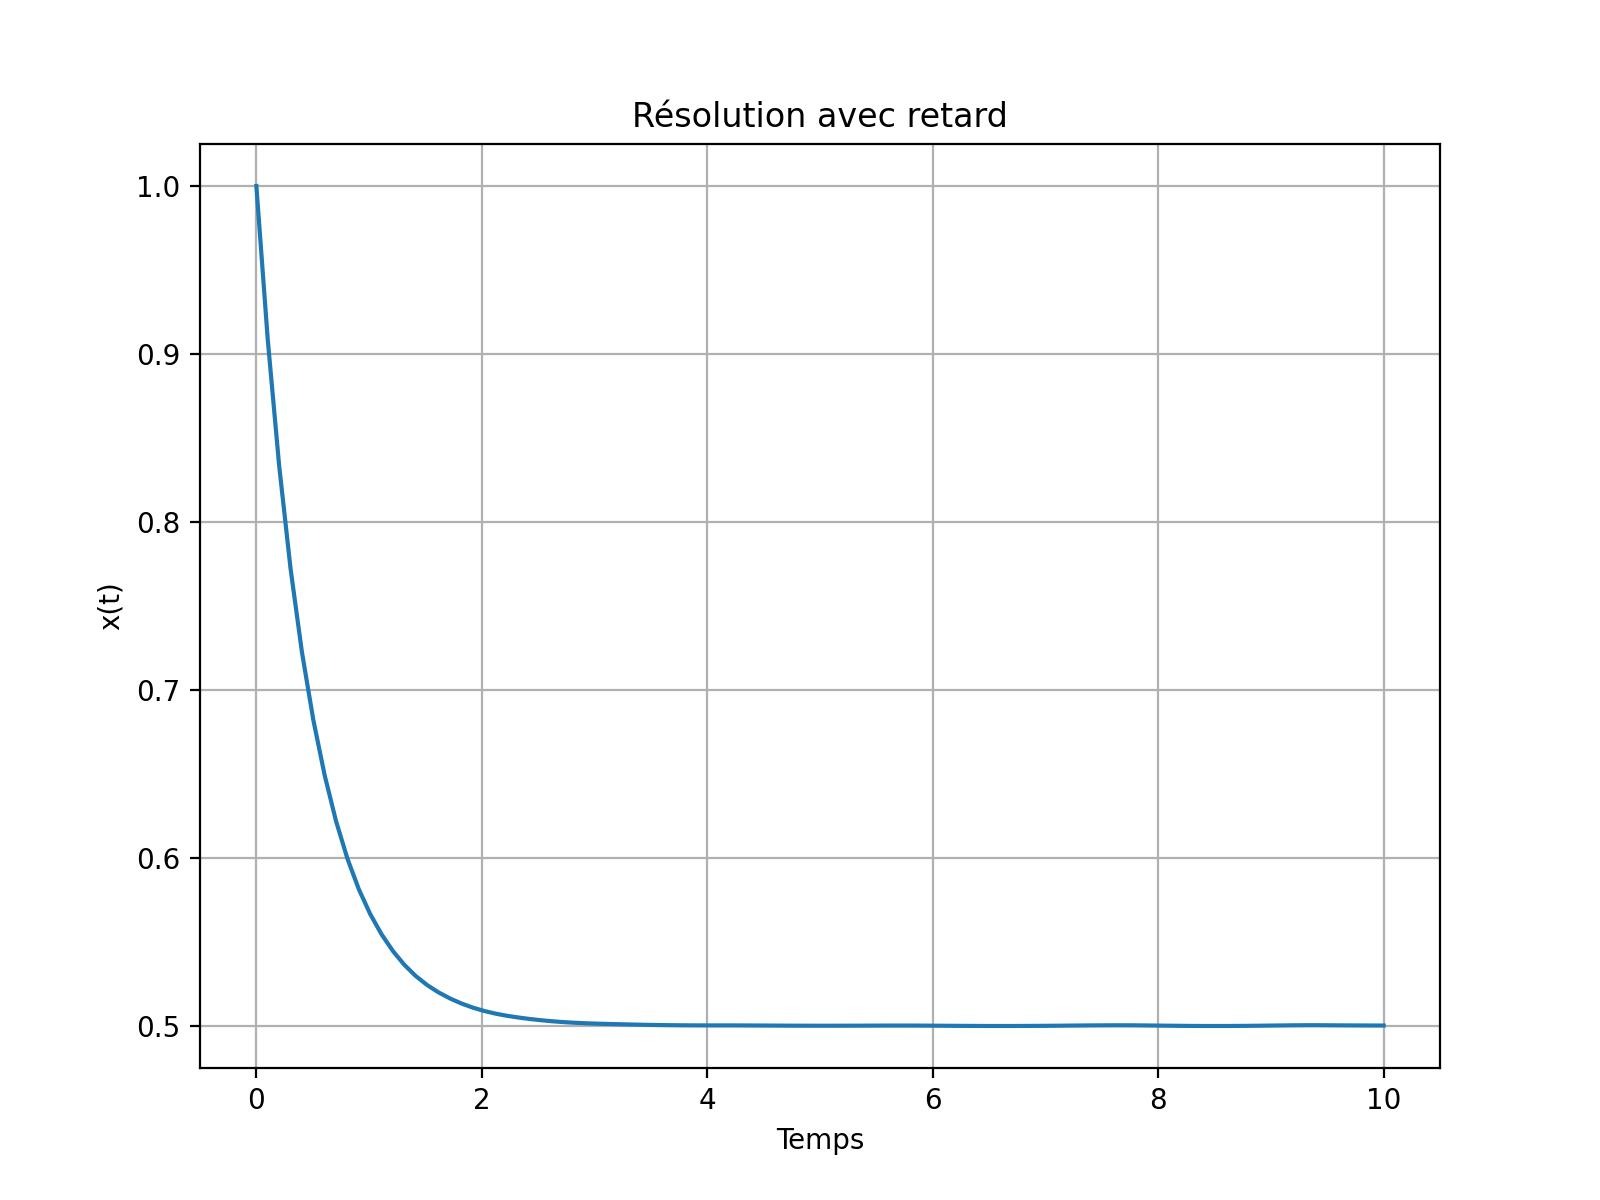
\includegraphics[width=\textwidth]{images/retard.jpg}
                    \caption{Solution numérique du système avec retard}
                    \label{fig:retard}
                \end{figure}

        \subsection{Croissance logistique}
            Le modèle logistique est largement utilisé pour représenter la croissance de populations soumises à une capacité limite \footnote{\url{https://fr.wikipedia.org/wiki/Fonction_logistique_(Verhulst)}}:
            \begin{equation*}
            \begin{cases}
            x'(t)=c\,x(t)\left(1-\frac{x(t)}{k}\right)\\
            y(t)=x(t)
            \end{cases}
            \end{equation*}
            Les conditions sont:
            \begin{itemize}
                \item Condition initiale: $x(0)=0.3$,
                \item Paramètres: $k=1.5$, $c=0.2$,
                \item Intervalle temporel: $[0,50]$.
            \end{itemize}
        
            \subsubsection{Solution numérique}
                Ce code montre la convergence vers la capacité limite du modèle logistique. Le graphique est présenté en Figure \ref{fig:logistique}.
                \inputminted{python}{codes/logistique.py}
                \begin{figure}[ht!]
                    \centering
                    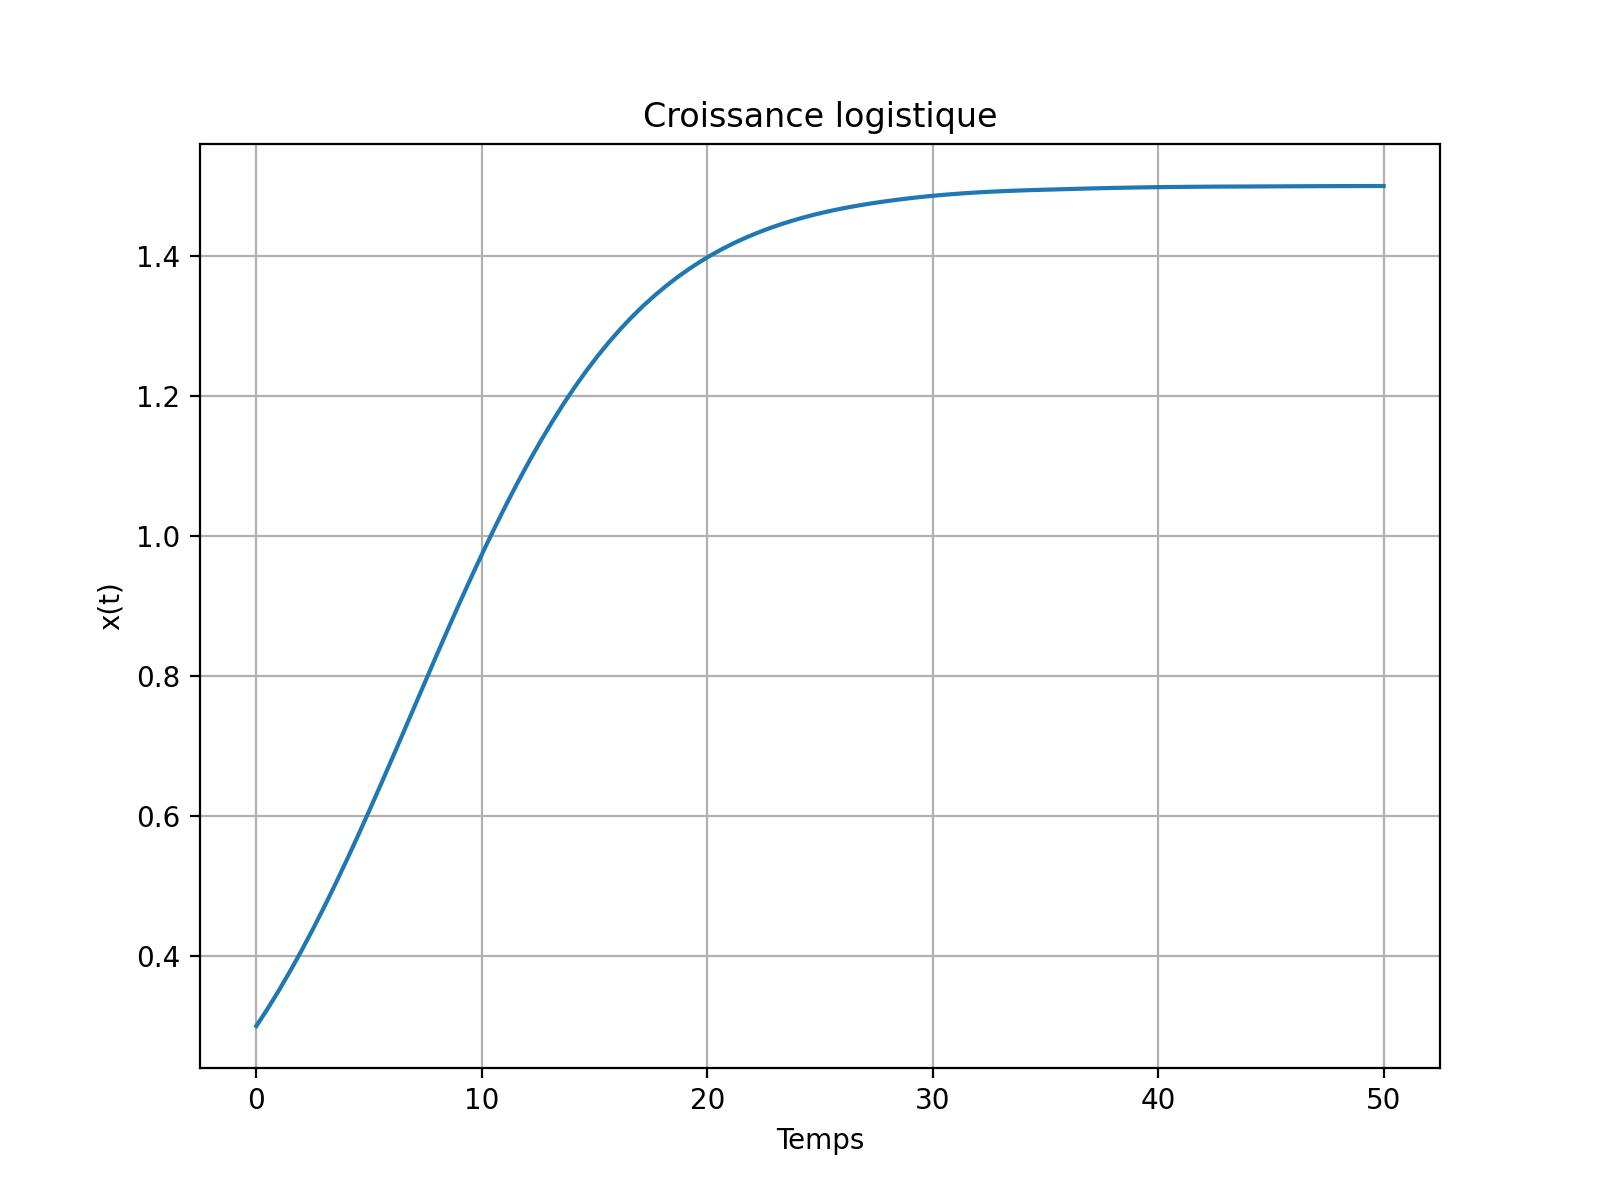
\includegraphics[width=\textwidth]{images/logistique.jpg}
                    \caption{Solution du modèle de croissance logistique}
                    \label{fig:logistique}
                \end{figure}
                
                En variant les conditions initiales, nous pouvons observer leur effet sur la dynamique de la population en Figure \ref{fig:logistique2}.
                \begin{figure}[ht!]
                    \centering
                    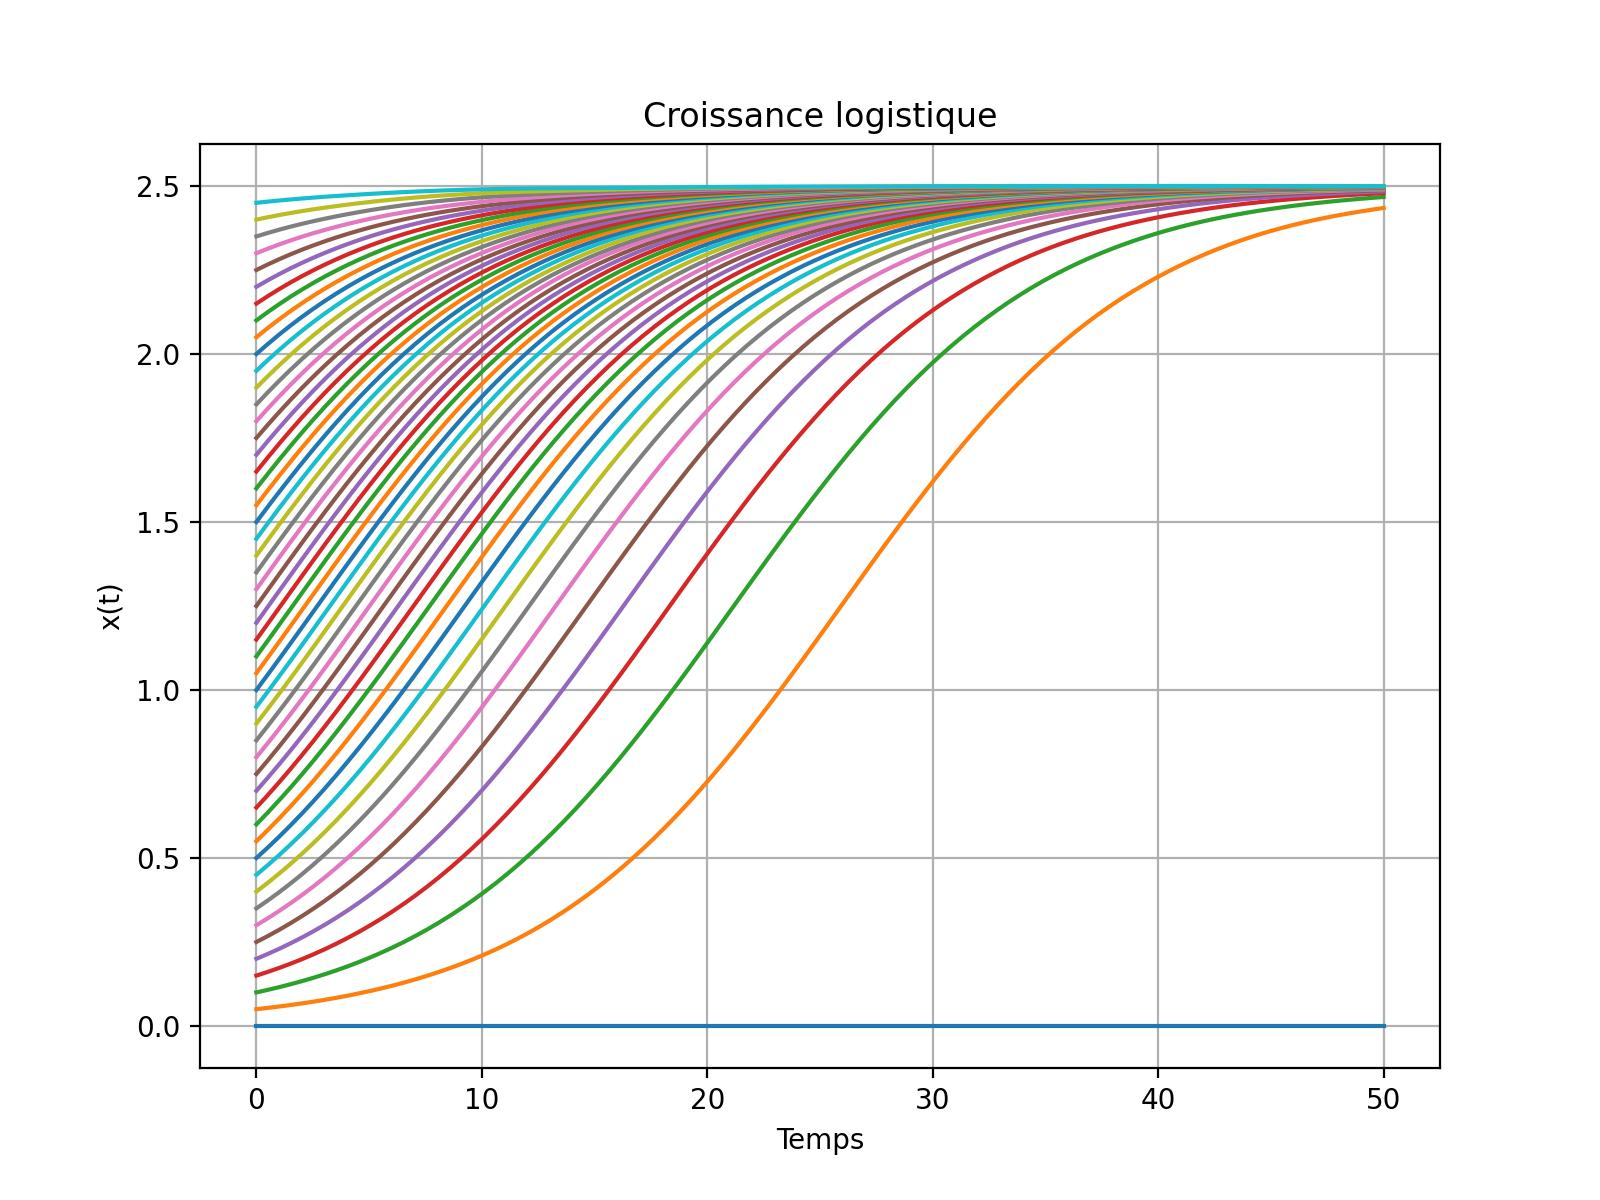
\includegraphics[width=\textwidth]{images/logistique2.jpg}
                    \caption{Effet des conditions initiales sur la croissance logistique}
                    \label{fig:logistique2}
                \end{figure}
    \section{Simulation de systèmes linéaires d'ordre 2}
        Les étapes pour la simulation et le dessin de portrait de phases des systèmes d'ordre deux sont les mêmes que celles vues dans le chapitre \ref{chap:portrait_phases}. Pour un système
        \begin{equation*}
            x'(t) = A x(t)
        \end{equation*}
        Les étapes à suivre sont les suivantes
        \begin{enumerate}
            \item Dessin des droites invariantes (vecteurs propres)~;
            \item Dessin des isoclines~;
            \item Dessin de vecteurs vitesse~;
            \item Dessin de trajectoire.
        \end{enumerate}
        \subsection{Exercices}
            \subsubsection{Trajectoire}
                \begin{exercise}{Trajectoire}
                    Écrivez une fonction \codeword{trajectoire(A: list[list], interval: list[int], c_i: list[int])->None} qui prend en paramètre une matrice \codeword{A}, un intervalle de simulation et une condition initiale, et qui affiche la trajectoire dans le portrait de phase. Utilisez \codeword{Numpy}, \codeword{SciPy} et \codeword{matplotlib}.
                \end{exercise}
                La solution est donnée par le code suivant, dont le résultat pour la matrice
                \begin{equation*}
                    A = \begin{bmatrix}-2 & 1\\ 1 & -2\end{bmatrix}
                \end{equation*}
                est donné dans la figure \ref{fig:trajectoire}
                \inputminted{python}{codes/trajectoire.py}
                \begin{figure}[ht!]
                    \centering
                    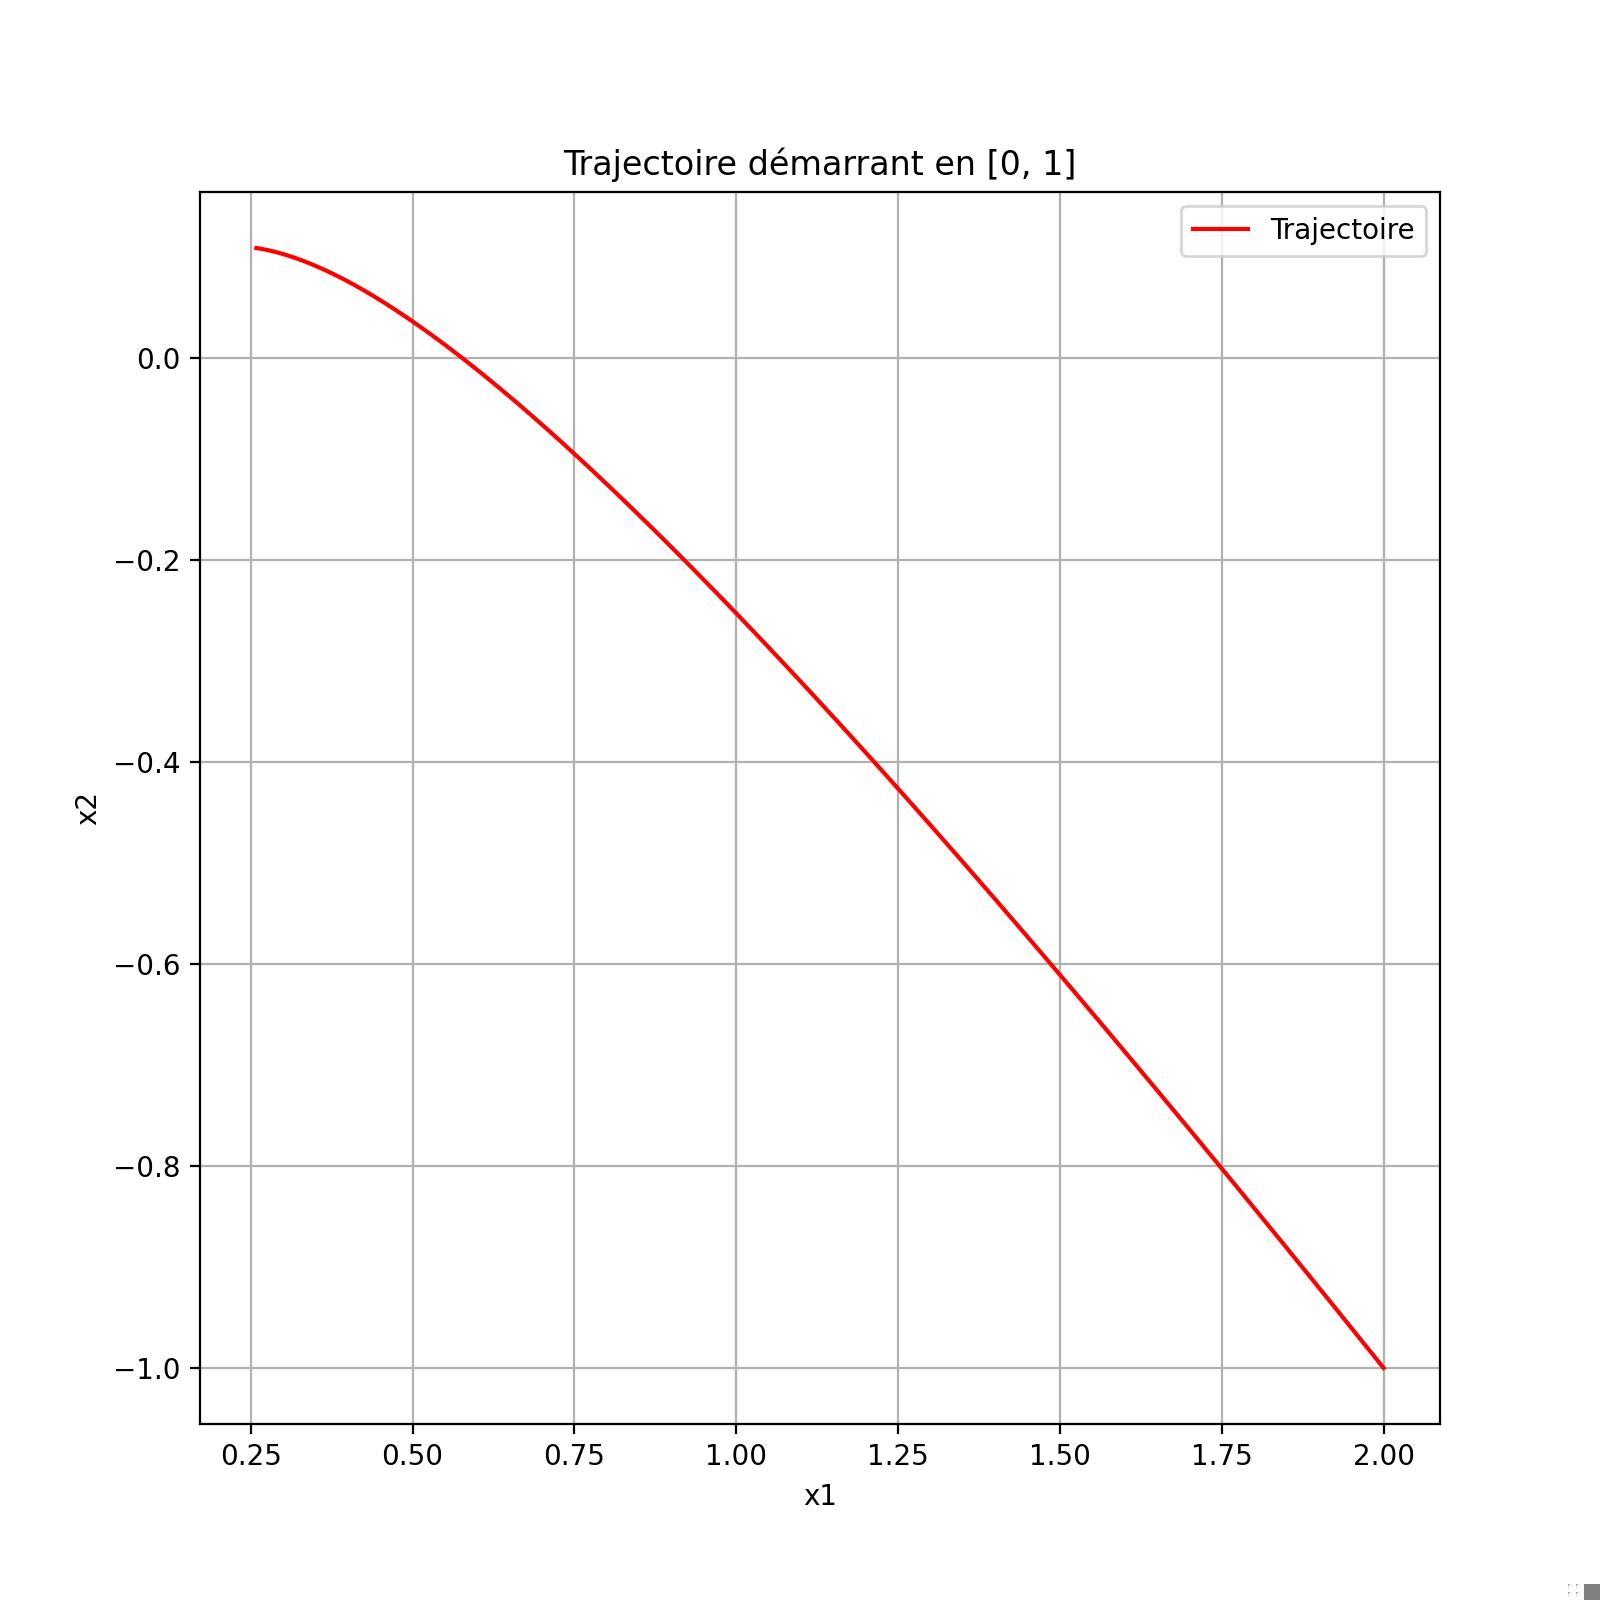
\includegraphics[width=\textwidth]{images/trajectoire.jpg}
                    \caption{Exemple de trajectoire}
                    \label{fig:trajectoire}
                \end{figure}
                
            \subsubsection{Vecteurs propres et droites invariantes}
                On veut dessiner plusieurs choses sur la même figure:
                \begin{itemize}
                    \item deux droites pour les vecteur propres~;
                    \item les flèches des vecteurs propres.
                \end{itemize}
                Pour dessiner les droites des vecteurs propres, il faut calculer la pente de la droite.
                Les vecteurs propres peuvent être calculés en utilisant la fonction \codeword{eig} du module \codeword{linalg} (pour \textit{linear algebra}) de \codeword{Numpy}.
                Les composantes de ces vecteurs propres peuvent être utilisés pour trouver la pente de la droite associée.

                \begin{exercise}{Vecteurs propres et droites invariantes}
                    Écrivez une fonction \codeword{vecteurs_propres(A: list[list])->None} qui prend en paramètre une matrice A et qui dessine les vecteurs propres et leurs droites associées.
                \end{exercise}
                
                La solution est donnée par le code suivant, dont le résultat pour la même matrice est donné dans la figure \ref{fig:invariants}
                \inputminted{python}{codes/invariants.py}
                \begin{figure}[ht!]
                    \centering
                    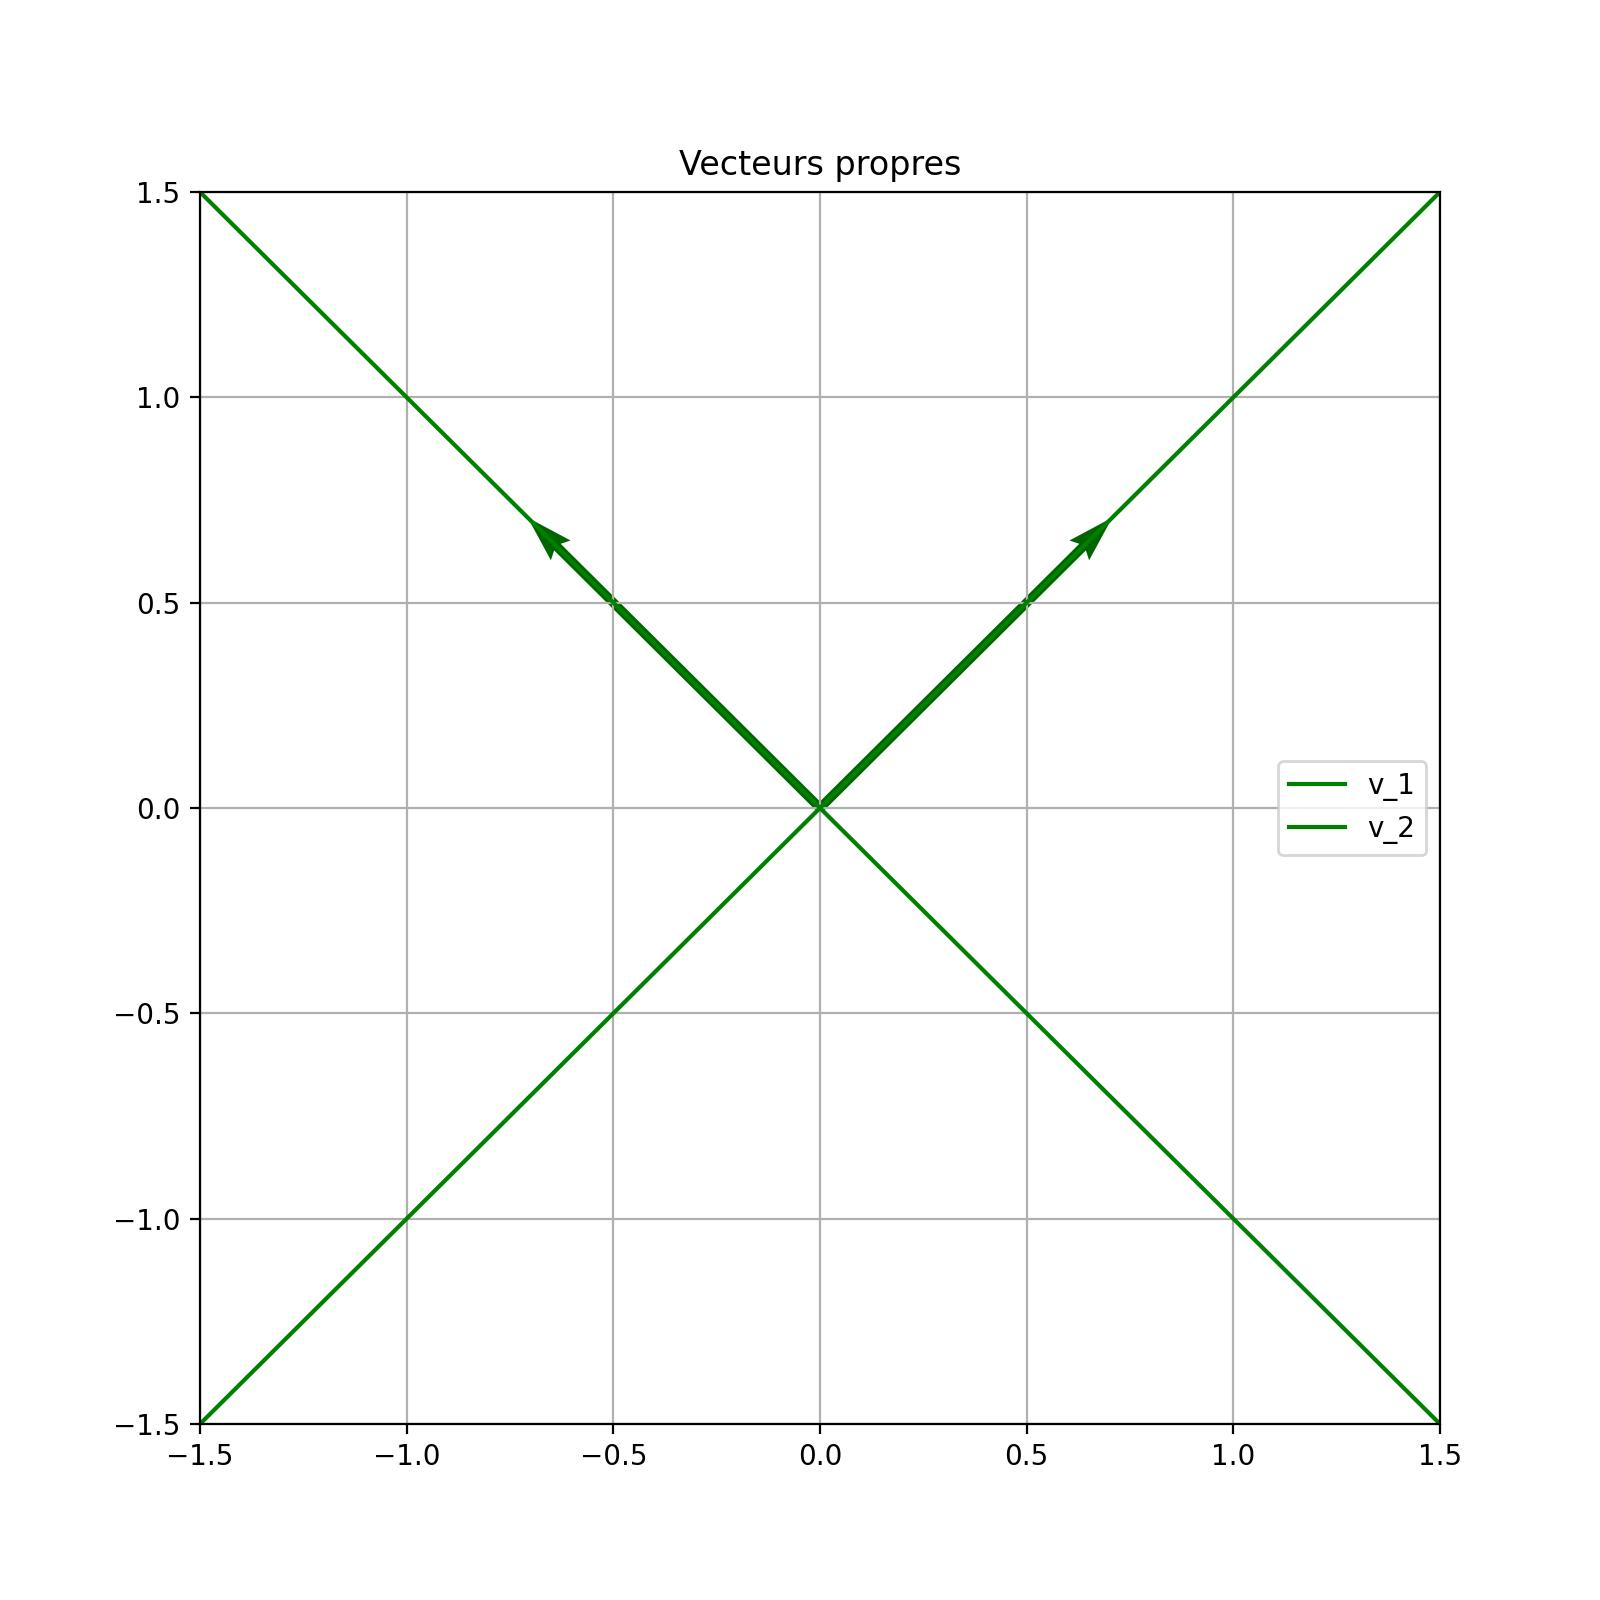
\includegraphics[width=\textwidth]{images/invariants.jpg}
                    \caption{Exemple de vecteurs propres et de droites invariantes}
                    \label{fig:invariants}
                \end{figure}

            \subsubsection{Isoclines}
                Le calcul des isoclines peut se faire d'une manière comparable aux vecteurs propres en exprimant $x_2$ en fonction de $x_1$.
                Comme
                \begin{equation*}
                    \begin{cases}
                        \dot{x_1} = a_{11}x_1 + a_{12} x_2\\
                        \dot{x_2} = a_{21}x_1 + a_{22} x_2
                    \end{cases}
                \end{equation*}
                
                Et que les isoclines sont la solution à \robin{Attention~: avec les accolades, on dirait que tu essayes de résoudre le système. Or si $A$ est inversible, la seule solution serait $x = [0, 0]^\top$ (qui est le seul ponit simultanément dans les deux isoclines)}~:
                
                \begin{equation*}
                    \begin{cases}
                        0 = a_{11}x_1 + a_{12} x_2\\
                        0 = a_{21}x_1 + a_{22} x_2
                    \end{cases}
                    \Longleftrightarrow
                    \begin{cases}
                        a_{12} x_2 = -a_{11}x_1\\
                        a_{22} x_2 = -a_{21}x_1
                    \end{cases}
                    \Longleftrightarrow
                    \begin{cases}
                        x_2 = -\frac{a_{11}}{a_{12}}x_1\\
                        x_2 = -\frac{a_{21}}{a_{22}}x_1
                    \end{cases}
                \end{equation*}
                Ce qui nous donne une pente de $-\frac{a_{11}}{a_{12}}$ et $-\frac{a_{21}}{a_{22}}$ respectivement.

                \begin{exercise}{Isoclines}
                    Écrivez une fonction \codeword{isoclines(A: list[list])->None} qui prend en paramètre une matrice A et qui dessine les isoclines associées.
                \end{exercise}
                
                La solution est donnée par le code suivant, dont le résultat est donné dans la figure \ref{fig:isoclines2}.
                \inputminted{python}{codes/isoclines.py}
                \begin{figure}[ht!]
                    \centering
                    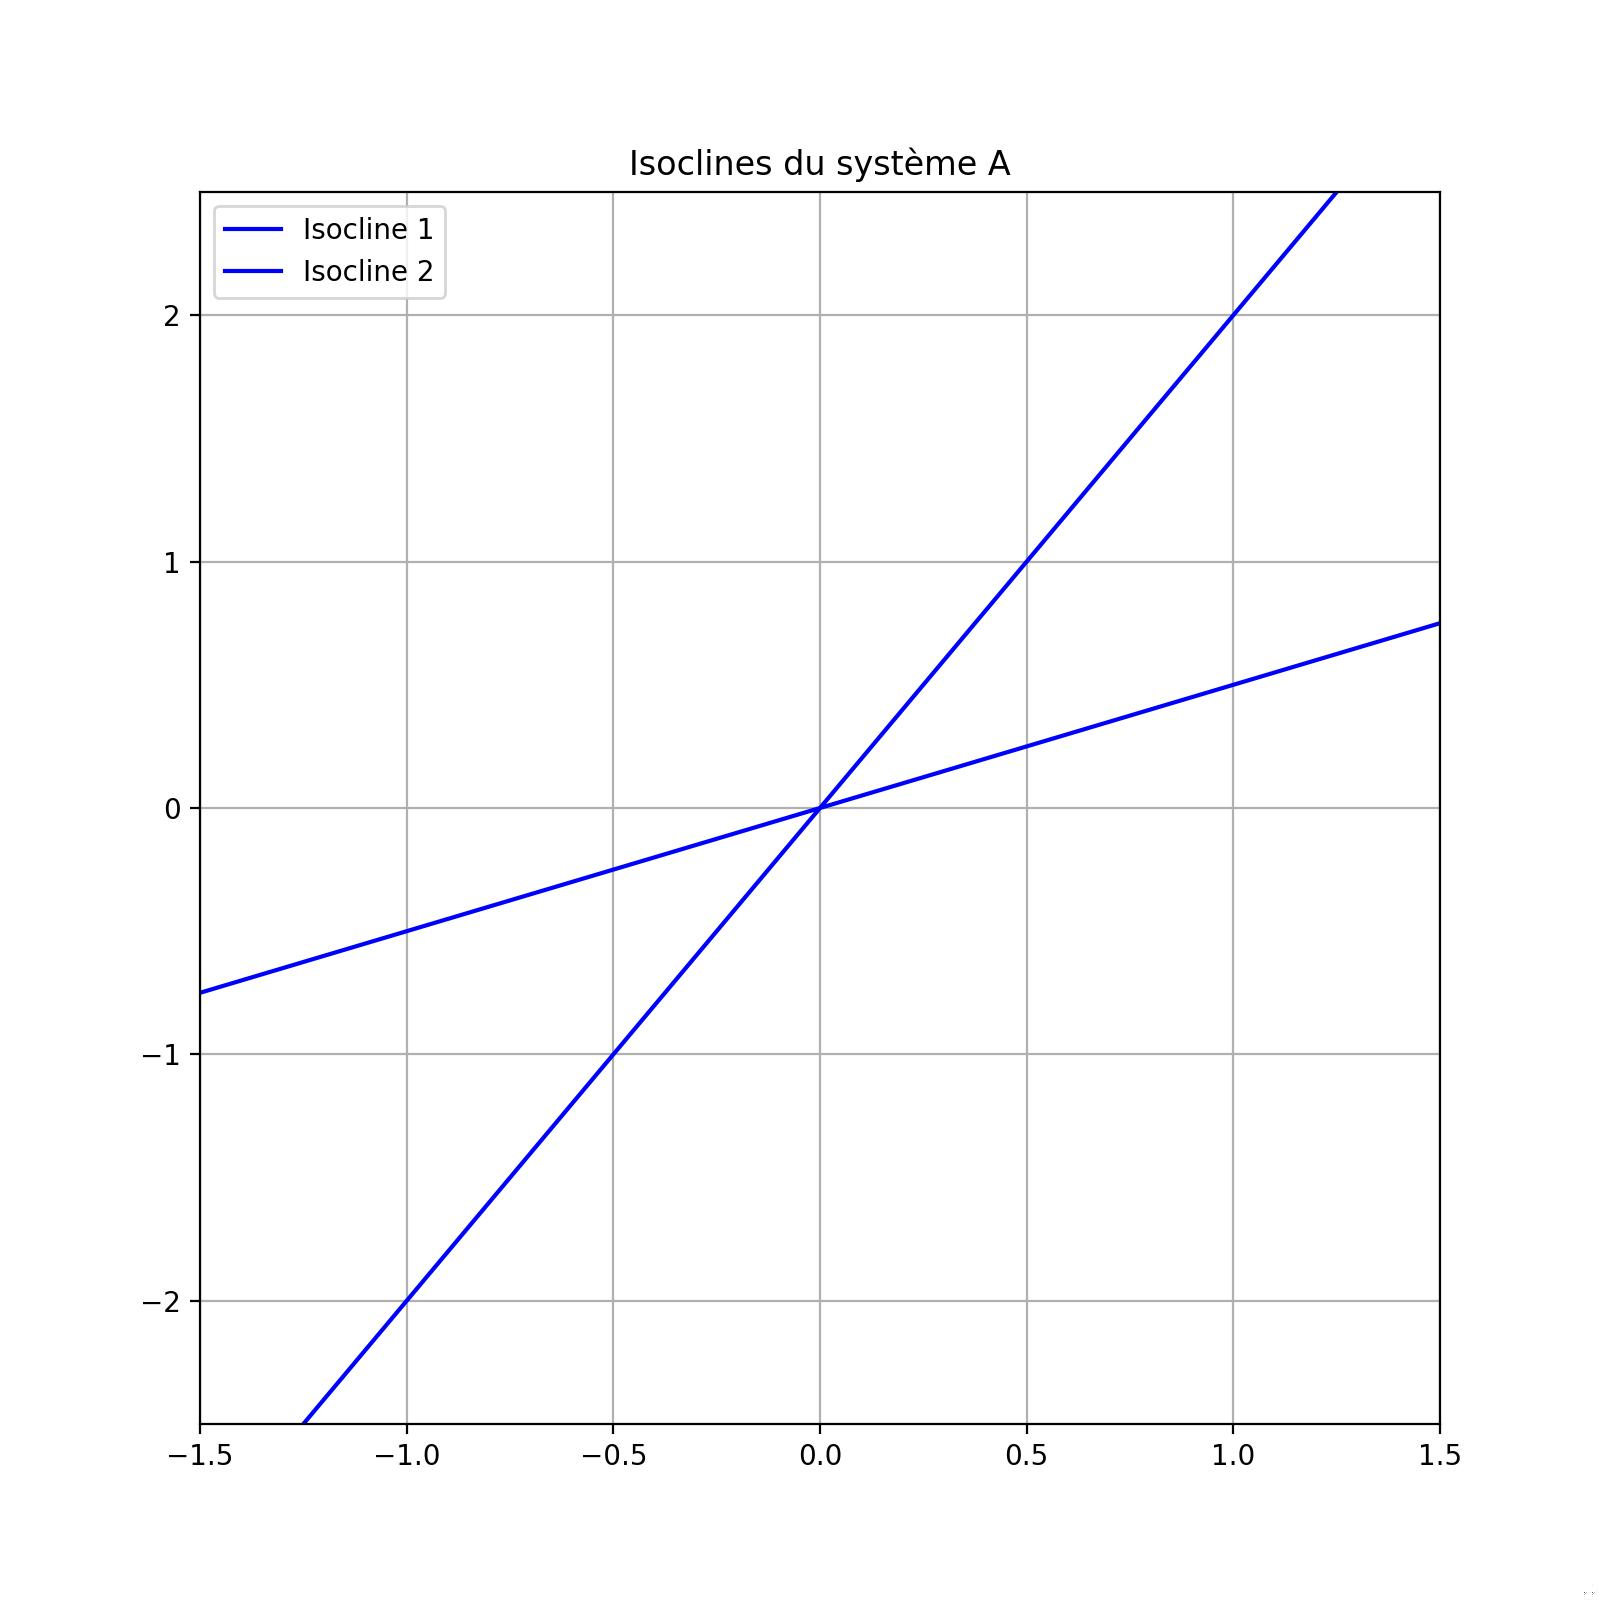
\includegraphics[width=\textwidth]{images/isoclines2.jpg}
                    \caption{Exemple d'isoclines}
                    \label{fig:isoclines2}
                \end{figure}
                
            \subsubsection{Champ de vecteurs vitesse}
                \begin{exercise}{Champ de vecteurs vitesse}
                    Écrivez une fonction \codeword{vecteurs_vitesse(A: list[list])->None} qui prend en paramètre une matrice A et un intervalle, et qui affiche le portrait de phase, pour tous les points situés sur une grille de taille de case $0.2$.
                \end{exercise}

                La solution est donnée par le code suivant, dont le résultat est donné dans la figure \ref{fig:champ_vecteurs_vitesse}.
                \inputminted{python}{codes/champ_vecteurs_vitesse.py}
                \begin{figure}[ht!]
                    \centering
                    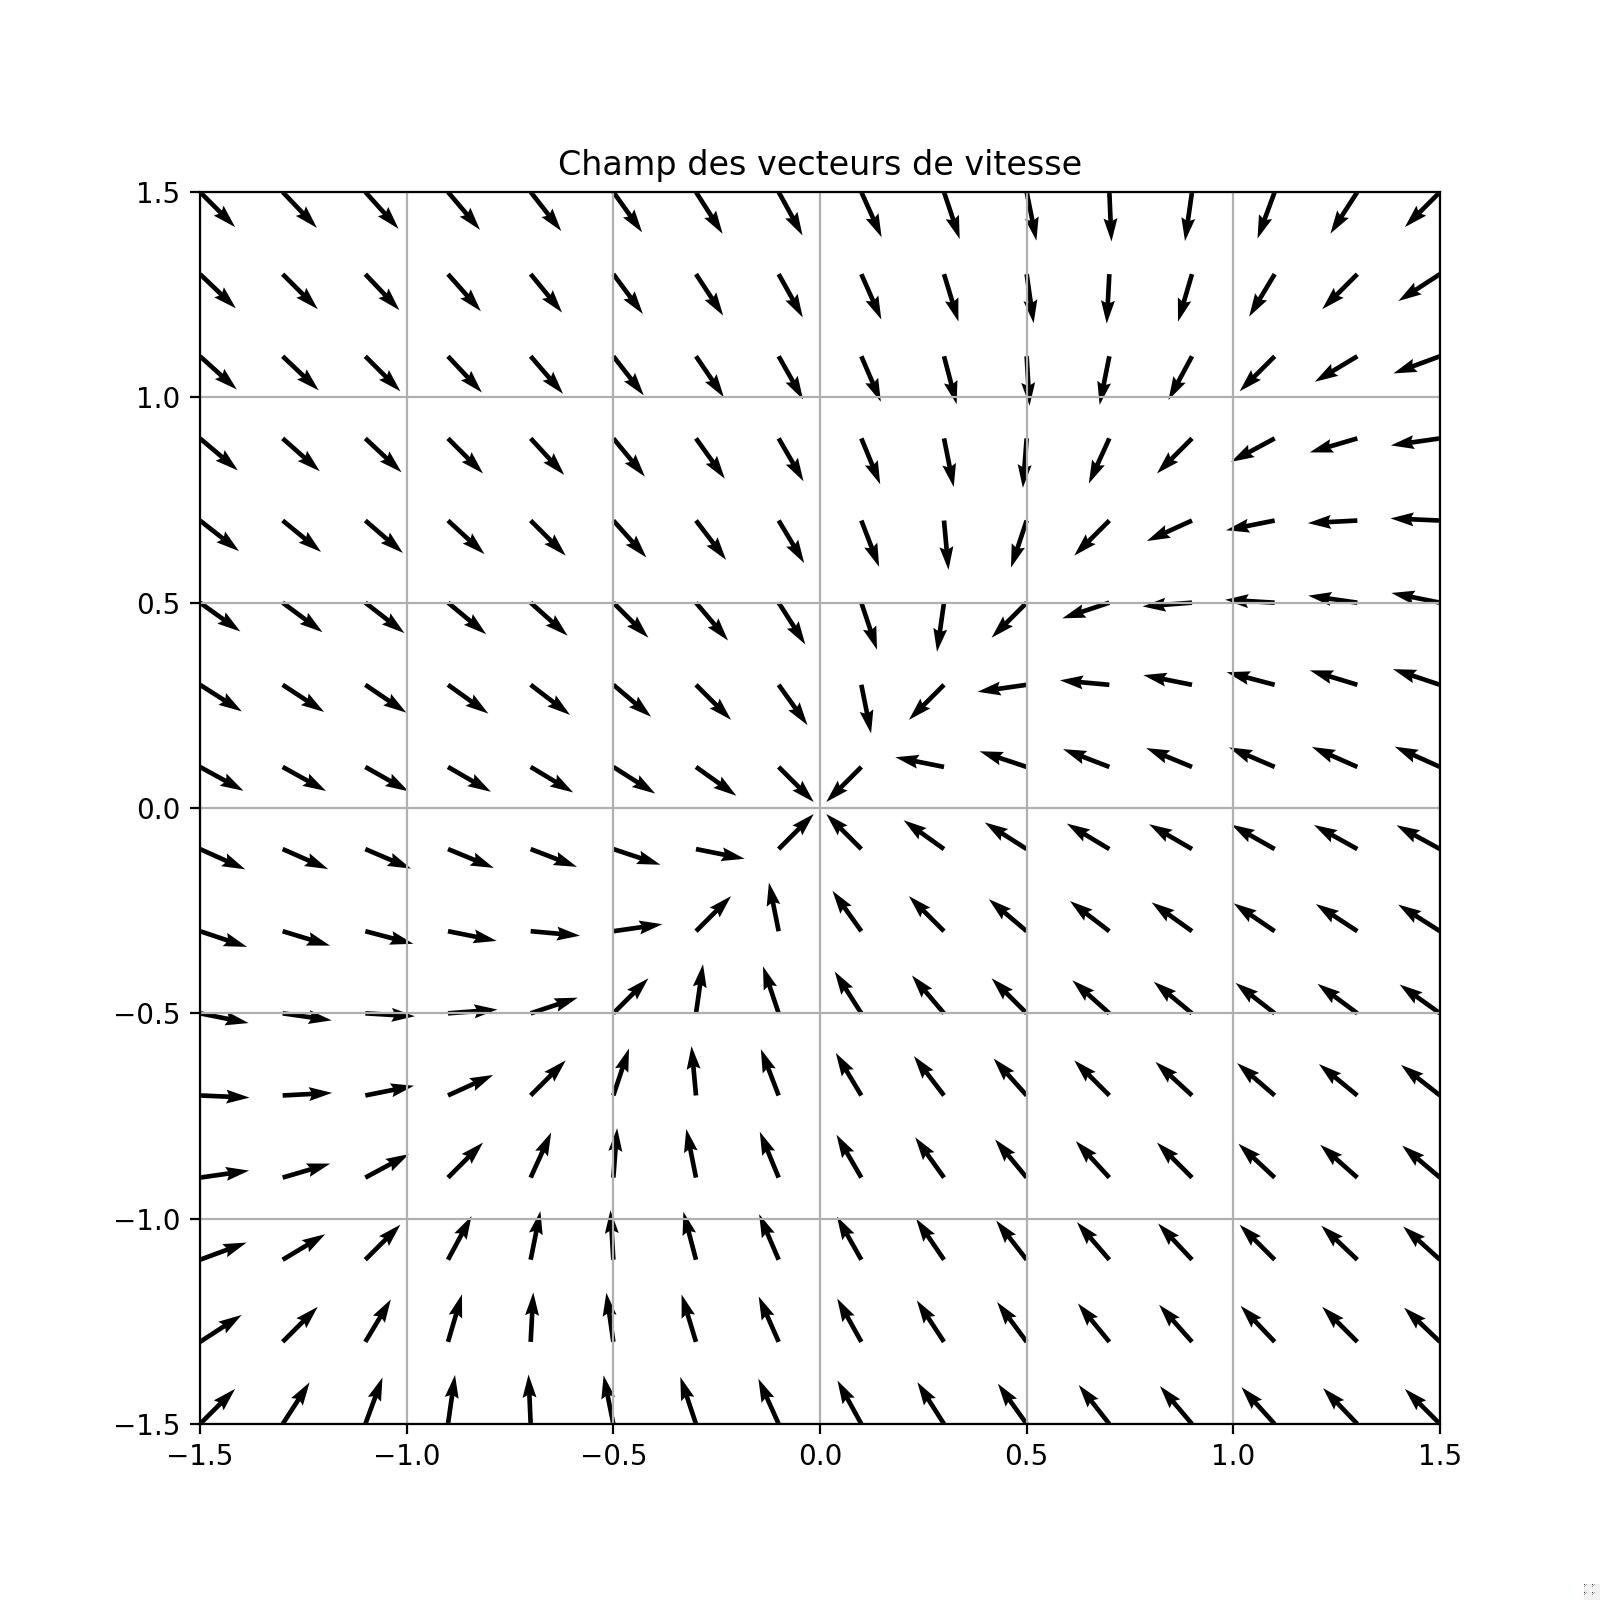
\includegraphics[width=\textwidth]{images/champ_vecteurs_vitesse.jpg}
                    \caption{Exemple de champ de vecteurs vitesse}
                    \label{fig:champ_vecteurs_vitesse}
                \end{figure}
                
            \subsubsection{Portrait de phases complet}
                \begin{exercise}{Portrait de phases}
                    Écrivez une fonction qui assemble tout le portrait de phase~:
                    \begin{itemize}
                        \item le champ de vecteurs~;
                        \item quatre trajectoires choisies arbitrairement~;
                        \item les isoclines~;
                        \item les vecteurs propres et les droites invariantes.
                        %\item 
                    \end{itemize}
                \end{exercise}

                La solution finale est donnée par le code suivant, dont le résultat est donné dans la figure \ref{fig:portrait_de_phases}.
                \inputminted{python}{codes/portrait_de_phases.py}
                \begin{figure}[ht!]
                    \centering
                    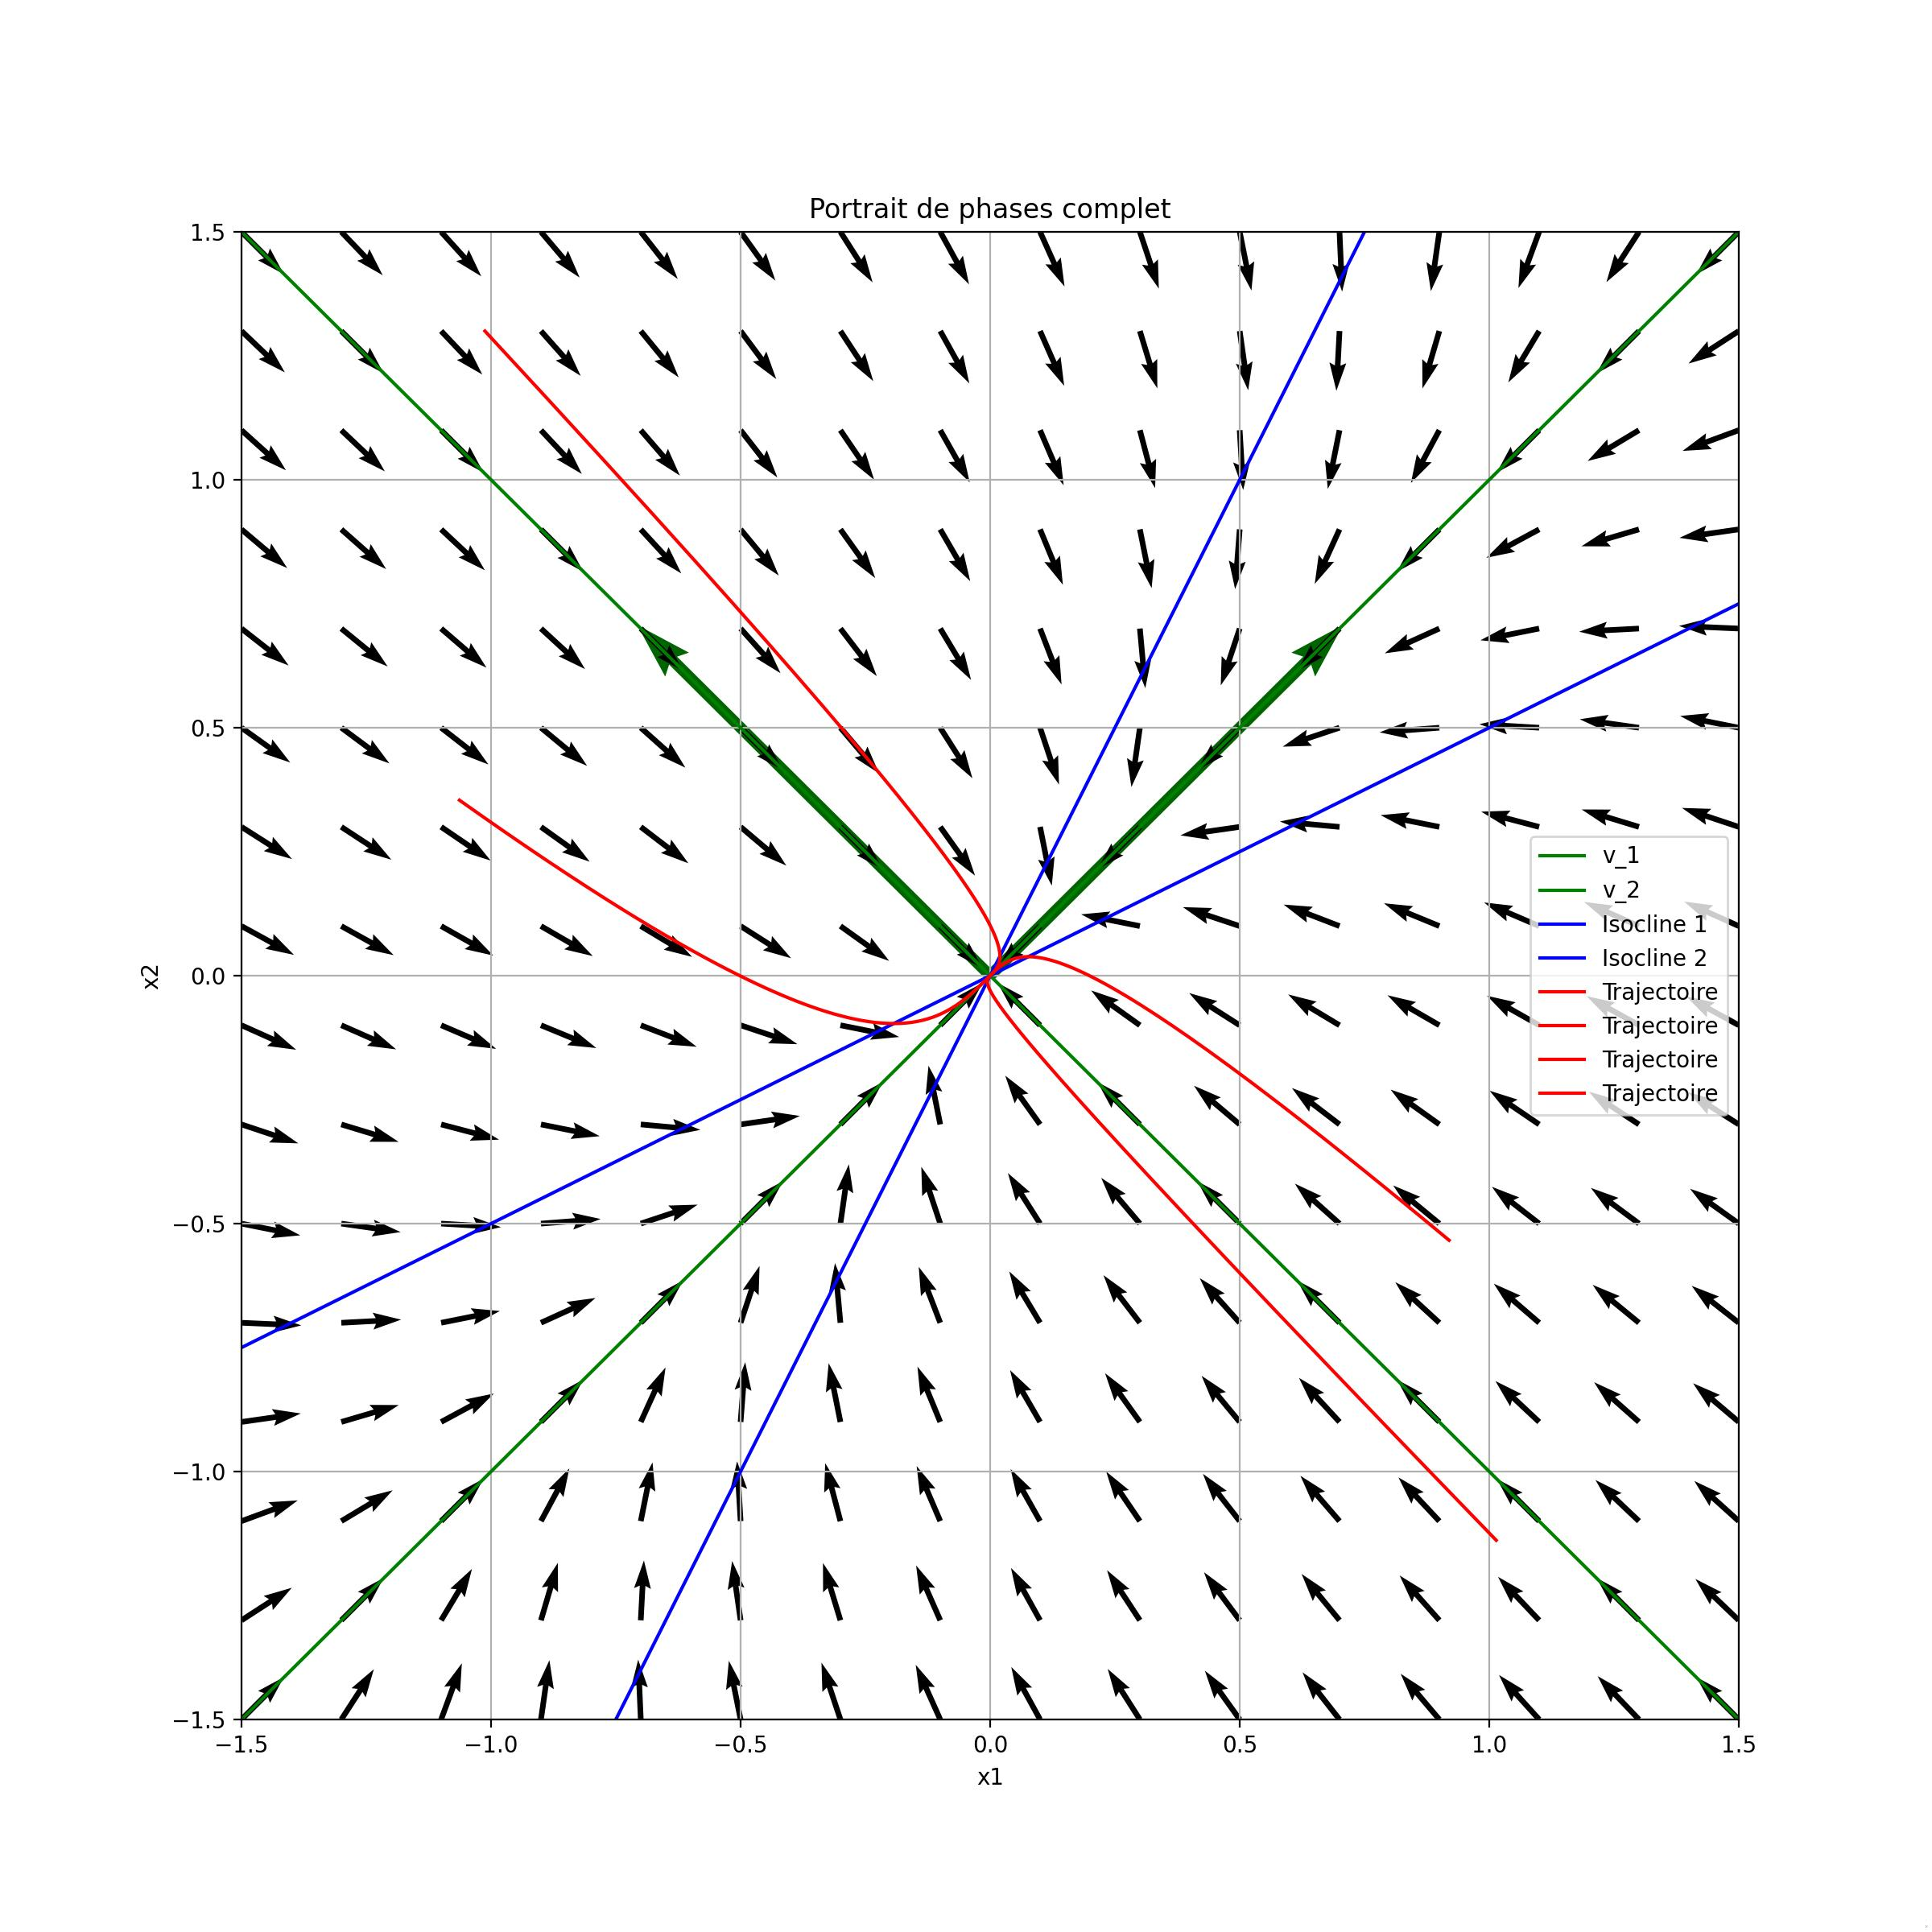
\includegraphics[width=\textwidth]{images/portrait_de_phases.jpg}
                    \caption{Exemple de portrait de phases}
                    \label{fig:portrait_de_phases}
                \end{figure}
    \section{Pour aller plus loin}
        Maintenant que le dessin de portrait de phases pour des systèmes linéaires d'ordre 2 a été extensivement abordé, il reste évidemment à aborder les systèmes non-linéaires. En pratique, la méthode reste la même que pour les systèmes linéaires, car la méthode de solution numérique s'applique aussi aux systèmes non-linéaires. Évidemment, certains raccourcis de calculs utilisés dans ce chapitre ne fonctionneront plus \textit{tels quels}: par exemple, le dessin d'une isocline ne sera vraisemblablement pas une droite. Certaines autres fonctions, comme celle du champ des vecteurs vitesses, peuvent être utilisées quelle que soit la (non-)linéarité du système, pour autant qu'il soit d'ordre 2.

        Pour les systèmes qui dépassent l'ordre 2, le défi technique devient alors la visualisation: le choix dépendra alors de l'application. Il vaudra mieux, parfois, afficher les trajectoires selon un sous-ensemble de paires de variables, ou préférer les animations. Ceci dépasse cependant le cadre de ce syllabus.